\documentclass[DM,lsstdraft,SDP]{lsstdoc}
%Replace the CUx here and all \CU will resolve below.

\usepackage{gwp}
\usepackage{risk}

\begin{document}

\setDocTitle    [DM Charter\CU]
                    {\color[rgb]{0.16,0.42,0.57} \sf Data Management Organization Charter 
                    }
\setDocAuthor   {William O'Mullane, Marion Juric, Jeffrey P Kantor,  Tim Axelrod,  Roberta Allsman}                % the author(s) \setDocApprove  {LSST Project Oeefice}              % approval by ...
\setDocRef      {LDM-294} % the reference code
\setDocIssue    {2}                        % the issue
\setDocRevision {1}                        % the revision
\setDocDate     {\today}              % the date of the issue
\setDocStatus   {draft}                    % the document status

%
% a short abstract
%
\setDocAbstract {This is the DM plan updaed from the v2 of 2014.
   It covers the organisation anfd managemnt of DM for LSST.}

\setDocCompact{true}

%
% the title page
%
\mktitle

%
%   Revision history
%
% MOST RECENT FIRST
\begin{docHistory}
\addtohist{2}{1}{2017-01-09}{WOM,MJ}{Update in TeX}
\addtohist{2}{0}{2015-03-11}{JK}{Updated with new RFC process, realignment of TCT, SAT, DMLT - other versions in between}
\addtohist{1}{1}{2004-06-23}{JK}{Initial version} 
\end{docHistory}

%
%   TOC
%
\newpage
\setcounter{tocdepth}{3}
\tableofcontents
\newpage

%
% It's all yours from here on
%


\frame{\frametitle{ A little about myself}
\begin{itemize}
\item 1985ish Life started with BASIC on a  commodore 
\item 1993 graduated  Computer Science Degree and Masters University College Cork, Ireland 
\item 1993 - 1997 Spacecraft Control Systems (C++) in ESA Mission Operations Centre Darmstadt Germany
\item 1997 - 2001 Hipparcos, Integral, Planck, Gaia, Bepi-Sax  (C,Java,Oracle, HTM, HEALPix) in ESA Technology Research Centre Noordwijk Netherlands
\item 2001-2003 Commercial programming - some Astronomy (Java) 
\item 2003-2005 The Johns Hopkins, SDSS and National Virtual Observatory (C,C\#,Java,Sqlserver)
\item 2005-2014 Gaia Astrometric Solution and Science Operations (Java, Oracle, Intersystems Cache) 
\item 2012  PhD in Physics on Implementing the Gaia Astrometric Solution,  Barcelona University
\item 2014-2017 All ESA Science Ground Segments in Development
\end{itemize}
}

\frame{\frametitle{Induction to astronomy : HIP Catalogue}
1997/98 Hipparcos Java Tools - learning Astrometry
\url{http://www.cosmos.esa.int/web/hipparcos/java-tools}
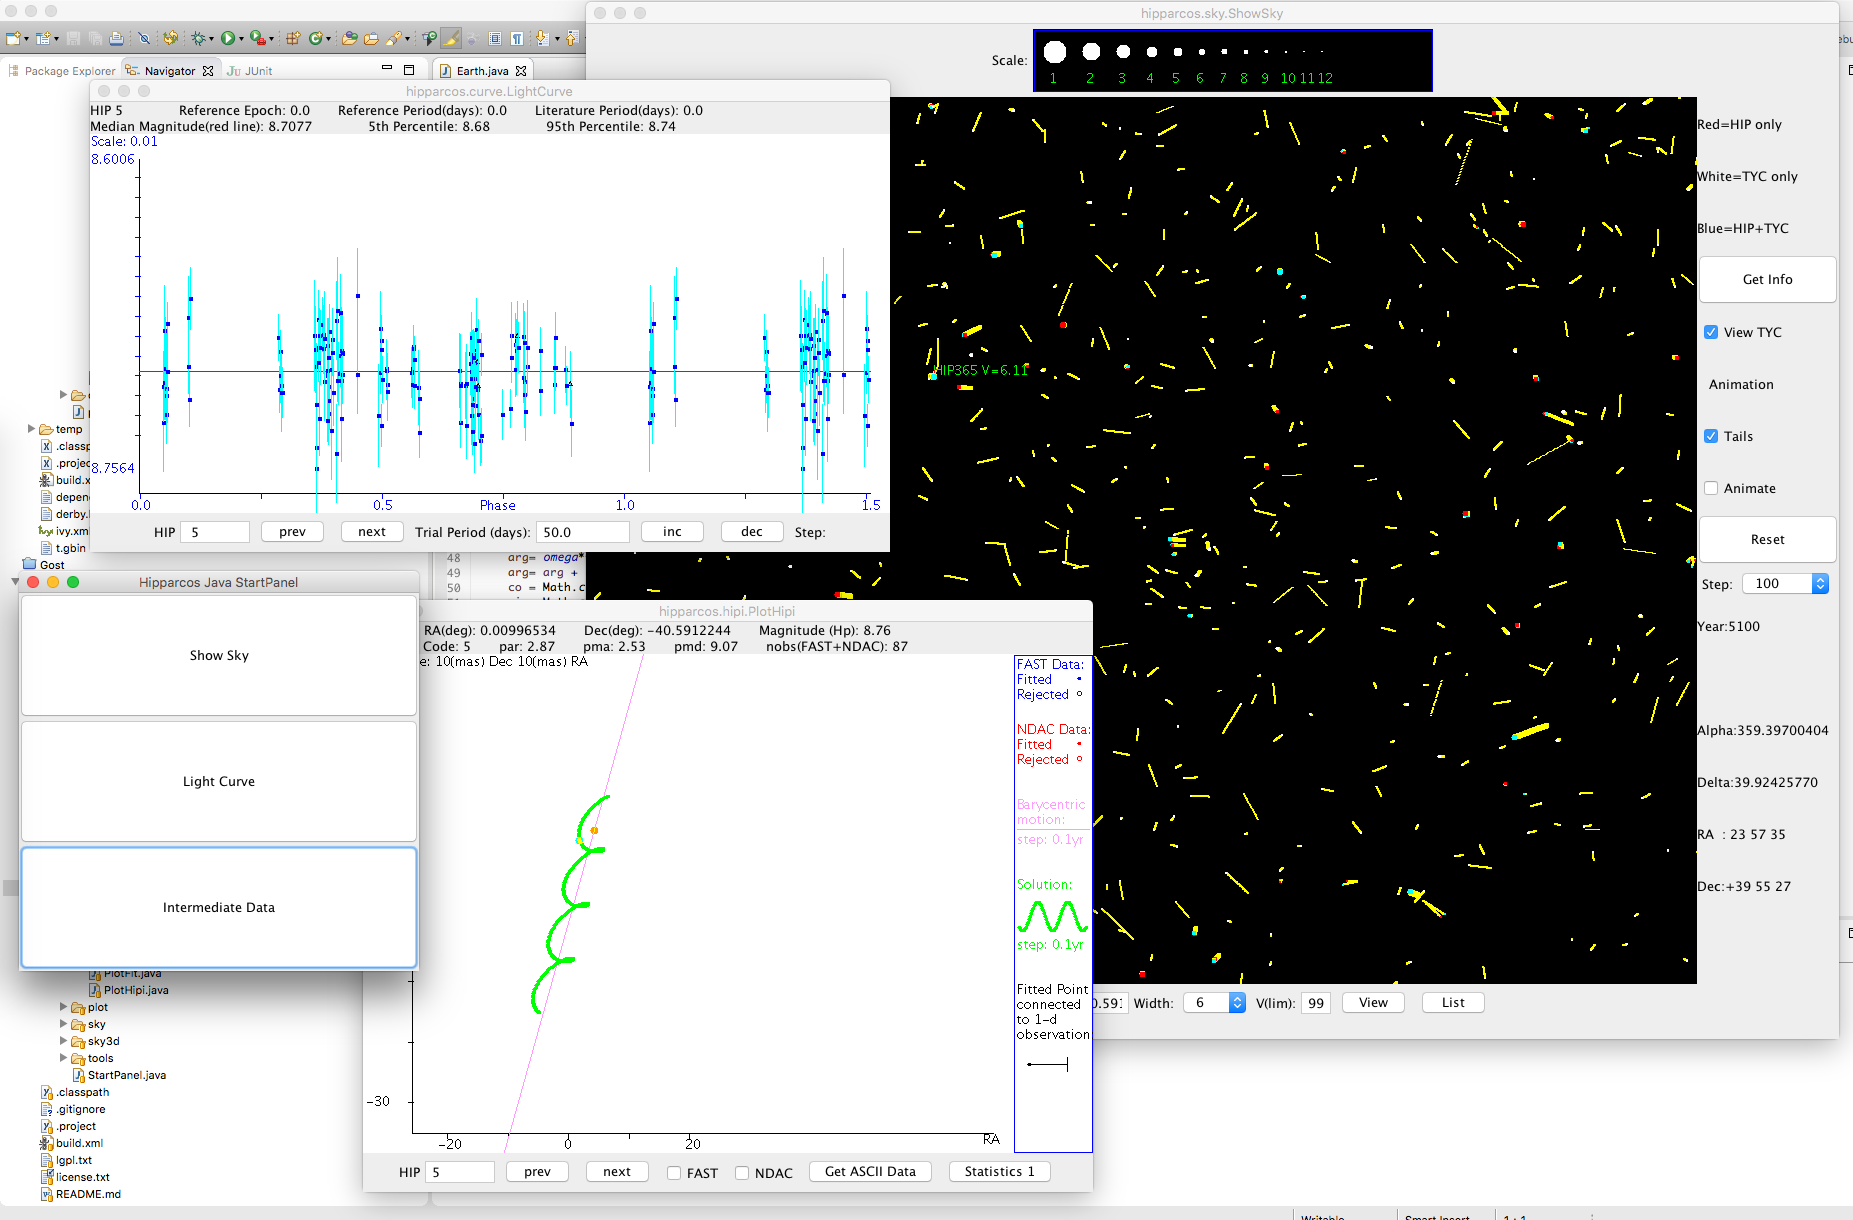
\includegraphics[width=\textwidth]{hipjt}
}

\frame{\frametitle{In the USA .. }
\vspace{5pt}
\begin{columns}[c]
\column{0.6\textwidth}
\vspace{4pt}
Quality tools for GSC2 (Java) $\rightarrow$\\
\vspace{8pt}
CasJobs (C\#)\citep{conf:casjobs}
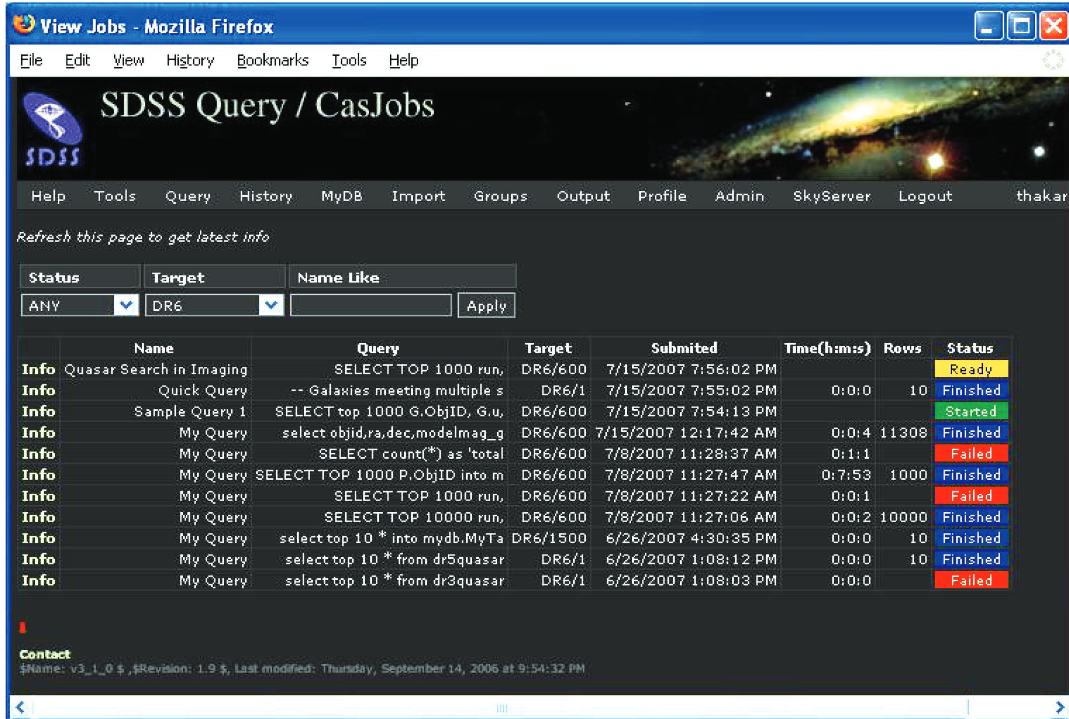
\includegraphics[width=\textwidth]{casjobs}
\column{0.4\textwidth}
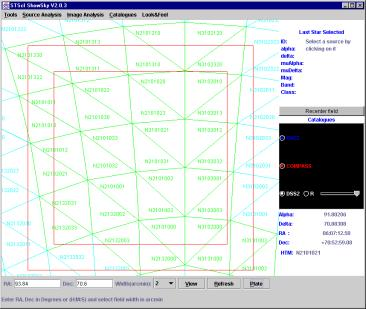
\includegraphics[width=\textwidth]{sshtm}
\vspace{-1cm}
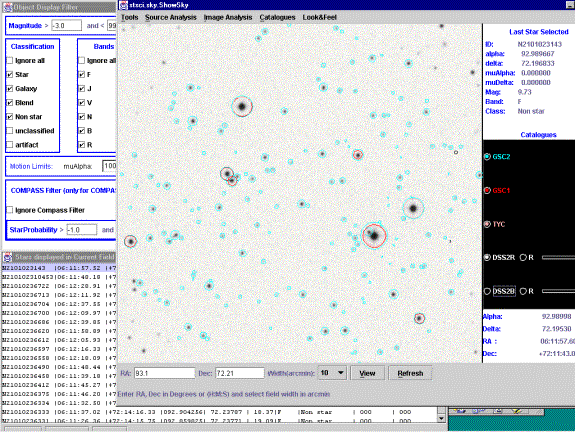
\includegraphics[width=\textwidth]{showsky}
\end{columns}
}


\frame{\frametitle{European Space Astronomy Centre }
\begin{columns}[c]
\column{0.4\textwidth}

\includegraphics[width=0.9\textwidth]{exm}\\

\includegraphics[width=0.45\textwidth]{bepiclogo}
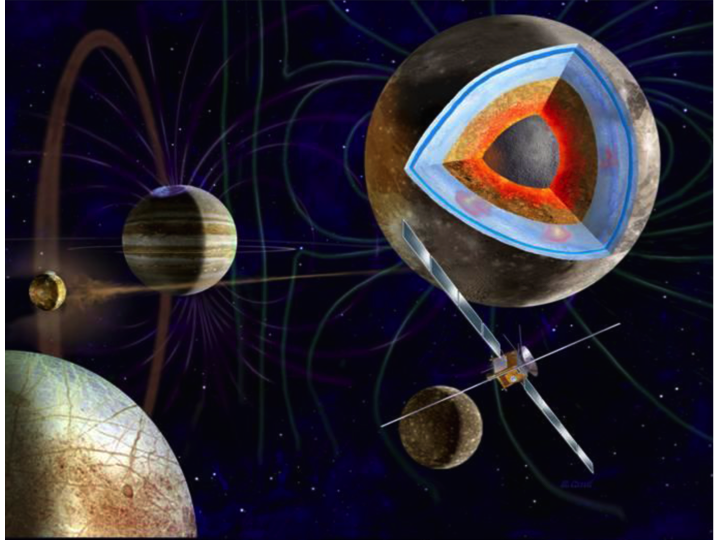
\includegraphics[width=0.45\textwidth]{juice}\\
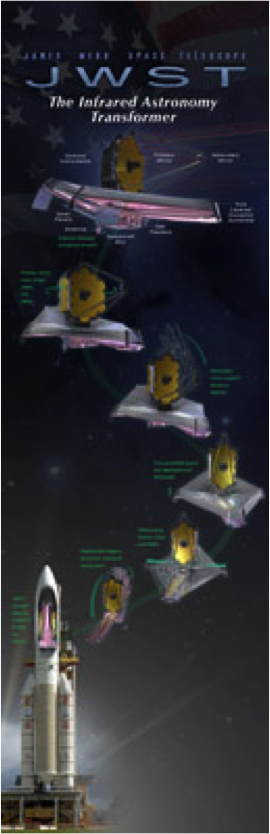
\includegraphics[width=0.45\textwidth]{jwst}\\
\vspace{-6cm}
\hspace{2.2cm}
\includegraphics[width=0.45\textwidth]{solo}\\
\hspace{2.2cm}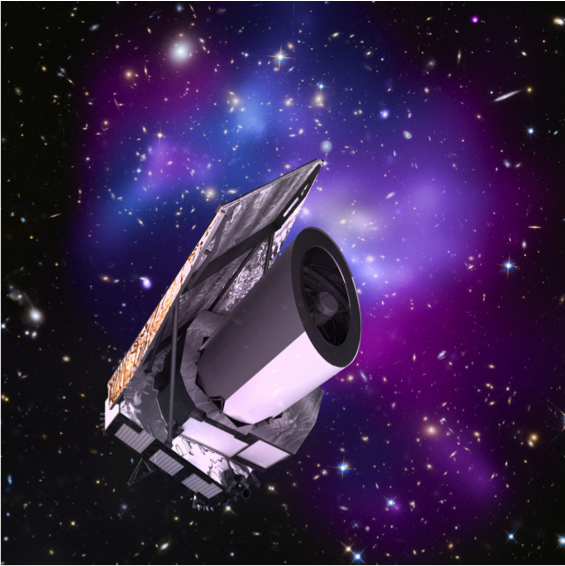
\includegraphics[width=0.45\textwidth]{euclid}

\column{0.6\textwidth}
\begin{itemize}
\item ESAC Located near Madrid, Spain.
\item Home of the Science Operations Department  containing  Operations Development Division.
\item Develop Science Operations Systems:
\begin{itemize}
\item People, Procedures and Software.
\item Interactions MOC and scientific communities.
\item Quite a bit of software - diverse - mainly Java but FORTRAN, C, C++, Python ..
\item Prepare for planning, simulations, instrument performance, commanding.
\item Hand over system to operations division after commissioning.

\end{itemize}
\end{itemize}
\end{columns}
}




\frame {\frametitle{ Data management }
    \begin{itemize}
	\item Victor remains interim PM until April 
	\item Have been trying to get an idea of DM organisation - talking to DMLT and TCAMS 
	\item Following are some observations and draft ideas 

    \end{itemize}

    {\bf   Look out for a  new version of LDM-294 - DM Management Plan}
    \begin{itemize}
	\item It will detail roles and responsibilities in DM
    \end{itemize}
    \vspace{12pt}
    DM Mission :\\
    {\em  Stand up operable, maintainable, quality services to deliver high-quality LSST data products for sciencer, all on time and within reasonable cost.}
}


\frame {\frametitle{ DM Organisation}

      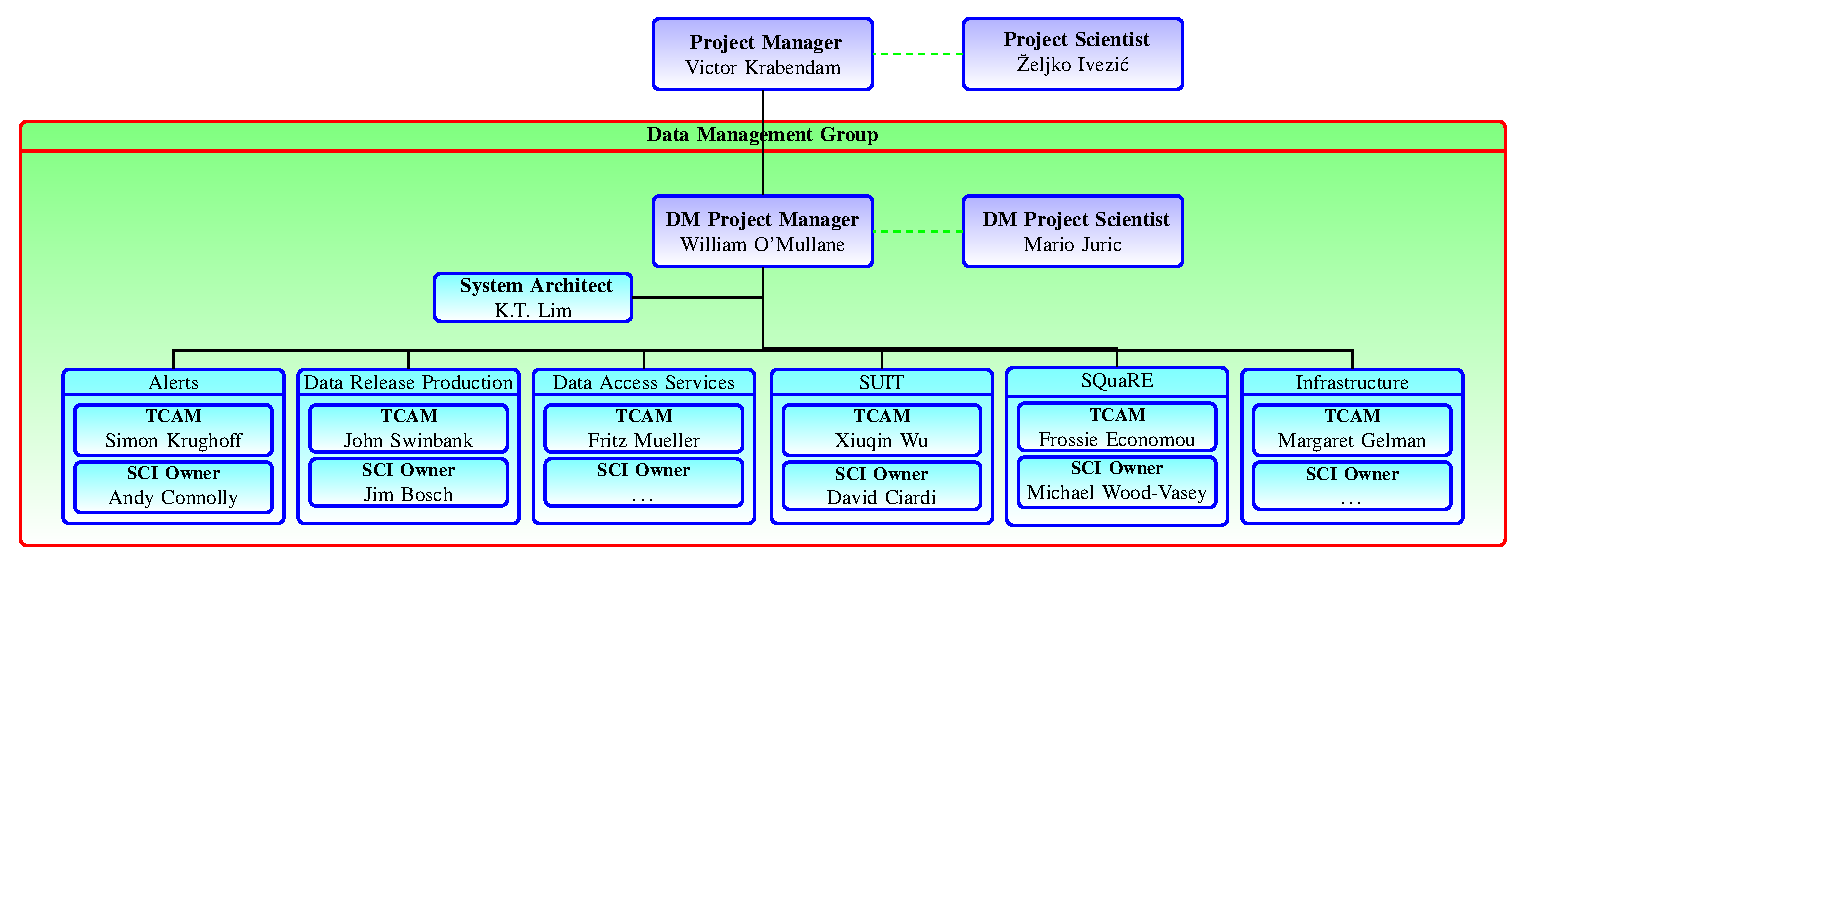
\includegraphics[width=1.0\textwidth]{images/DmOrg}\\
}

\frame {\frametitle{ DM architecture \& products}
	\begin{itemize}
	\item Would like to get  a list of products in DM
	\item Related to understanding the DM architecture - KT working on LDM-148 update more from him in a while
	\item Those are not Data Products - mostly Systems and Software artefacts
	\item For each product identify {\em Product Owner} and manager.
	\item This would change the org chart ..
	
	\end{itemize}

}

\frame {\frametitle{ Risk Management and other processes ..}
Also in LDM-294:
	\begin{itemize}
	 \item Would like an open Risk approach - anyone can raise a risk (Tim working on that)	
	 \item Document management - in next slid as
	 \item Configuration control 
	 \item Product assurance  and Scientific Validation 
	\item \ldots
	\end{itemize}
Mainly these will be high level and point to the details in other documents. 

}

\section{Data Management Problem Management/Escalation}
The above organizational structure allocates significant responsibility to lead institutions.  As such, when problems arise that cannot be solved with the responsibility and scope allocated to an institution, the path of escalation and resolution of such problems must be clear.  In cases of problems that cannot be solved within the DM organization, that escalation path must also be clear.  \figref{fig:probman}  depicts the escalation path for such problem resolution.


\begin{figure}[htbp]
\begin{center}
 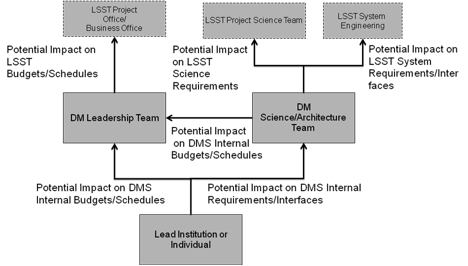
\includegraphics[width=0.8\textwidth]{images/probman}
\caption{Problem Management/Escalation\label{fig:probman}}
\end{center}
\end{figure}


\section{Data Management Senior Positions and Responsibilities}
LSST Data Management Managers and Staff
These individuals form the top level management of the DMO.
DM Project Manager
The DM Project Manager is responsible for the efficient coordination of all LSST activities and responsibilities assigned to the DMO. The DM Project Manager has the responsibility of establishing the organization, resources, and work assignments to provide DM solutions.  The DM Project Manager, serves as the DMO representative in the LSST Project Office and in that role is responsible for presenting DM initiative status and submitting new DM initiatives for approval consideration. Ultimately, the DM Project Manager, in conjunction with his / her peer Project Managers (Telescope, Camera), is responsible for delivering an integrated LSST system. The DM Project Manager reports to the LSST Project Manager. Specific responsibilities include:

\begin{itemize}
\item Manage the overall DM System
\item Define scope and funding for DM System 
\item Develop and implement the DM project management and control process, including earned value management
\item Approve the DM Work Breakdown Structure (WBS), budgets and resource estimates
\item Participate in identification of new DM partners 
\item Approve or execute as appropriate all DM outsourcing contracts 
\item Convene and/or participate in all DM reviews
\item Co-Chair the DM Leadership Team
\end{itemize}
DM Deputy Project Manager
The DM Deputy Project Manager, if this position is implemented, assists the DM Project Manager in the efficient coordination of all LSST activities and responsibilities assigned to the DMO.  Specific responsibilities are the same as the DM Project Manager, when delegated to the DM Deputy Project Manager by the DM Project Manager.
DM Project Scientist
The DM Project Scientist has ultimate responsibility for ensuring DMO initiatives provide solutions that meet the overall LSST scientific and technical requirements.  The DM Project Scientist must ensure correct specification of DM Scientific Requirements and proper translation of those requirements into derived information technology requirements and ultimately, into implemented solutions.  The DM Project Scientist must ensure that the DM subsystem is properly scoped and integrated within the overall LSST system.  The DM Project Scientist is also a member of the LSST Project Science Team (PST) and reports to the LSST Director. Specific responsibilities include:

\begin{itemize}
\item Responsible for the science deliverables of the DM System
\item Set requirements for the DMS that:
\end{itemize}
o Ensure that the design and operational flow of the data products meet the needs of the science community
o Ensure that the quality requirements of the data products will be / are being met by the DMS, with a particular emphasis on choice of appropriate application algorithms
\begin{itemize}
\item Set requirements for and assess/validate results of Data Challenges and other precursor experiments
\item Set requirements and assess/validate results for Data Releases
\item Convene and/or participate in all DM reviews
\item Co-Chair the DM Leadership Team and Science/Architecture Team
\end{itemize}
DM Science Quality and Reliability Engineering (SQuaRE) Leads
The DM SQuaRE Leads are the SQuaRE Lead Scientist and the SQuaRE Technical Manager.  The primary organizational responsibility for this Tucson-led group is to provide scientific and technical feedback to the LSST DM Manager that demonstrates LSST/AURA DM is fulfilling its responsibilities as charged by the NSF with regards to science quality and software/IT performance and reliability.
They are responsible for monitoring the reliability and maintainability of software developed by DM and the quality of the data products produced by the DM software in production. SQuaRE's activities span processes and environments for software development, integration test and distribution.  SQuaRE also assumes responsibility for delivering any work in this area, though in many cases this may involve effort across the DM team. 
As such, areas of activity include:
\begin{itemize}
\item Development of algorithms to detect and analyze quality issues with data
\item Infrastructure development to support the generation, collection, and analysis of data quality and performance metrics
\item DM developer support services to ensure DM is using appropriate tools to aid software quality
\item Support of publicly released software products, including porting and distributing it according to the scientific community?s needs.
\end{itemize}

In the event that SQuaRE identifies issues with the performance or future maintainability of the DM codebase, it brings them to the attention of the DM System Architect, who is ultimately responsible to decide who will address them and how. In the event that SQuaRE identifies issues with the quality of the data, it brings them to the attention of the DM Project Scientist. 
DM System Architect
The DM System Architect is responsible for ensuring that all elements of the DM systems, including infrastructure, middleware, applications, and interfaces, adhere to a documented, integrated architecture, consistent with the overall LSST systems architecture.  The DM System Architect reports to the DM Project Manager and DM Project Scientist. Specific responsibilities include:
\begin{itemize}
\item Responsible for the overall design integrity of the DMS as a system, including
\end{itemize}
o Internal and external interfaces and overall architecture
o Use of frameworks and off-the-shelf components
o Sound engineering practice
\begin{itemize}
\item Ensure that the DMS design is traceable to an meets the requirements set by the DM Project Scientist, through requirements/design models and technical reviews
\item Set standards for development, implementation, and documentation of the DMS, and ensure that they are being met by all DM participants
\item Participate in stakeholder and end user coordination and approval processes and reviews
\item Member of the LSST System Engineering Team
\item Co-chair the DM Science/Architecture Team
\end{itemize}


\section{Lead Institution Senior Positions}
Each Lead Institution has a Project Manager and Scientific/Engineering Lead, who jointly have overall end product responsibility for a broad area of DM work, typically a Work Breakdown Structure (WBS) Level 2 element. They are supervisors of the team at that institution.  Their roles and responsibilities are similar to the DM Project Manager, DM Project Scientist, and DM System Architect, and DM QA and Test Lead, but within the scope of work assigned to that institution.  These leaders are bound to acknowledge and implement direction from the DM leadership in all matters pertaining to the DM project.  The DM Project Manager and DM Project Scientist have direct input into the performance appraisals of the Institution Project Manager and Scientific/Engineering Lead. 



\appendix
\section{DMO Discussion and Decision Making Process}

The Escalation process only occurs when the issue cannot be resolved within the DMO, i.e. when the following internal discussion and decision making process has failed to yield a decision.
Empowerment
All DMO team members are empowered by the DM Project Manager (PM) and Project Scientist (PS) to make decisions on any DM-internal matter, including technical/algorithm issues, process improvements, tool choices, etc., when:
A) they are willing and able to do the work to implement the decision or with people who agree with the team memaber,
B) they (collectively) are willing and able to fix any problems if it goes wrong, and
C) they believe that all affected parties (including your immediate manager) would not seriously object to your decision and implementation.
RFC Process
If the above three criteria are not met, perhaps because the team member doesn't know all the affected parties or because they don't know their positions, the team member should publish the proposed decision and implementation as a JIRA issue in the Request For Comments (RFC) project with a component of "DM".

It is usually difficult to determine all the affected parties for published package interfaces. Changes to interfaces should thus typically go through this process.

It's a good idea to contact any known affected parties before starting this process to check that the resolution is sensible. The institutional technical manager is always affected, as she or he is responsible for tracking the work schedule. If work for others is being proposed, they are obviously affected. The institutional scientist, the DM System Architect (SA), the DM Interface Scientist (IS), and the DM Project Scientist (PS) are also valuable resources for determining affected parties.

The purpose of an RFC is to inform others about the existence and content of the proposed decision and implementation in order to allow them to evaluate its impact, comment on it, refine it if necessary, and agree (implicitly or explicitly) or object (explicitly) to its execution.

The discussion of the RFC takes place in the medium of the requestor's choosing (e.g., a specific mailing list, the RFC JIRA issue itself, a HipChat room, a convened videocon, some combination of those, etc.), but the requestor should be open to private communications as well.

In the RFC process, the opinions of those who will be doing the work (and fixing any problems if something goes wrong) are given more weight. In some cases, this may mean that the RFC issue's Assignee passes to someone else. The opinions of more senior people or people more experienced in the area should also be given more weight and may also result in the Assignee changing.

The Assignee is responsible for determining when no serious objections remain.  In particular, there is no need to call for a formal vote on the (refined) resolution. If no explicit objections have been raised within, typically, 72 hours for "ordinary" issues and 1 week for "major" issues, the Assignee should assume that there are none. This is known as "lazy consensus". When this state has been reached, the Assignee is responsible for ensuring that the final consensus has been recorded in the RFC issue before closing it and proceeding with implementation of the decision.

The requestor must be especially careful about not making irreversible changes in the "lazy consensus" time period unless they are absolutely certain there's a general agreement on the stated course of action. If something is broken, the requestor must be be ready to fix it. It is critical to apply sound reasoning and good judgement about what may be acceptable and what might be not. Mistakes will happen; accept that occasionally there will be a requirement to revert an action for which it was thought agreement existed.
Exceptions and Appeals
Some proposed resolutions may require changes to one or more of the baselined, change-controlled documents describing the Data Management system (those in DocuShare with an LDM- handle or marked as change-controlled in Confluence).  Note that major changes to budget or scope will almost certainly affect one or more LDM- documents.  In this case only, the DM Technical Control Team (TCT), consisting of the DM PM, PS, SA, and IS, may empanel an ad hoc committee including the lead author of the document and other relevant experts. This committee or the TCT itself must *explicitly* approve the change.

Change-controlled documents with other handles, such as LSE- or LPM-, including inter-subsystem interfaces, have project-wide change control processes. Please consult the DM PM, SA, or IS for more information.
At least one member of the DM TCT will read each RFC to determine if it might affect a change-controlled document.

If the DMO team can't converge on a resolution to an RFC that has no serious objections but the requestor still feel that something must be done, the request will be escalated. In most non-trivial cases, they will, with the advice of the SA, empanel a group of experts to which they will delegate the right to make the decision, by voting if need be.

Formalities
For project management purposes, RFCs are formally proposals made to the DM PM and PS who by default are responsible for everything in DM (they "own" all problems). As owners, they have the final word in accepting or rejecting all proposals. Functionally, they delegate that ownership ? the right and responsibility to make decisions -- to others within the team (e.g. the SA, IS, group leads, etc.) who are expected to delegate it even further. Notifying the institutional technical manager about an RFC serves to inform the DM PM.


\section{Pre-Construction Phase Organization}\label{sect:precon}
This section is historical in nature and describes the DM Organization as it has evolved during the Conceptual, Preliminary, and Final Design Phases prior to Construction.
\subsection{Conceptual Design Phase}
As shown in \figref{fig:precon}
\footnote{LSST Science Council no longer exists. It has been replaced by the LSST Project Science Team and the LSST Science Advisory Committee }
, during the Conceptual Design Phase, the Project Manager and Project Scientist jointly supervise several Working Group, which are aligned by functional area.  The Working Group Leads are strictly technical leaders responsible for specific work areas, and have no budgetary or schedule authority.  Their primary work is the development of requirements and architecture in each of these functional areas.



\begin{figure}[htbp]
\begin{center}
 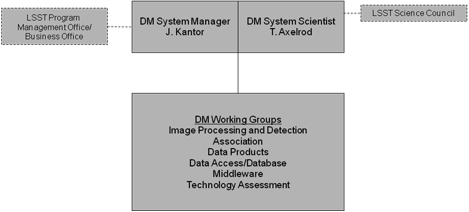
\includegraphics[width=0.8\textwidth]{images/precon}
\caption{Data Management Conceptual Design Phase Organization\label{fig:precon}}
\end{center}
\end{figure}

\subsection{
Preliminary Design Phase
}
The organization transitions to a more complex structure during Preliminary Design, as the role of each DM partner institution is solidified, and D\&D prototype development projects called Data Challenges become a primary organizing/tasking vehicle for D\&D work.  The Working Groups still remain and play a cross-institutional functional role in each area, but there is a more formal structure for work allocation and responsibility, as shown in \figref{fig:pdphase}.



\begin{figure}[htbp]
\begin{center}
 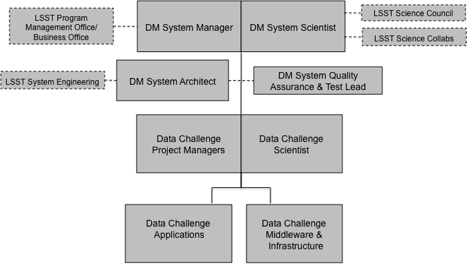
\includegraphics[width=0.8\textwidth]{images/pdphase}
\caption{ Data Management Preliminary Design Phase Organization\label{fig:pdphase}}
\end{center}
\end{figure}


In this phase, new positions reporting to the Project Manager and Project Scientist are added.  First, there is the DM System QA and Test Lead, who assists the Project Manager in preparation of formal plans, processes, and environments for software development, integration, and test. 
A Data Management System Architect supports the Project Manager and Project Scientist in matters related to LSST system engineering, including other subsystem interfaces, overall LSST system control, real-time external system interfaces (e.g. alerting), simulation, and end-to-end system engineering for quality assessment.
Finally, temporary Data Challenge Teams consisting of astronomers and engineers are formed for prototyping specific critical design aspects that have high risk (e.g. precursor and simulated data processing and prototype work, research and development of new algorithms for moving object detection or data distribution).  Each Data Challenge Team has a designated Project Manager who reports to the Project Manager and Scientist who reports to the Project Scientist for the duration of the Data Challenge.


\subsection{
Final Design Phase
}
During Final Design Phase, the organization structure transitions to one that will persist for the remainder of the period in which the DM System is developed and commissioned, up to the start of LSST Observatory operations.
As shown in \figref{fig:fdphase}, the organization now features lead institutions, each with responsibility for major element of the DM System (Level 2 Work Breakdown Structure elements) and Project Manager.  For example, during Final Design, the Processing Services/Tools and Archive Site Manager and Team at NCSA will be conducting prototyping activities in computing, data communications, and data storage to select and verify the ability of System technologies to support the LSST requirements.  They will also be involved in creating a supporting infrastructure for the DM Systems.  During Construction before the LSST first light time frame, these resources will be focused on implementation of the selected technologies.  In order to ensure that team functions as one integrated project, the institutions coordinate support by other lead institution team members directly through this organizational structure, as well as via a number of cross-organizational bodies (described later in this document). 
Also, due to the span of the organization, the DM Project Manager will be supported by one of the lead institution Project Managers as a Deputy Project Manager in these phases.


\begin{figure}[htbp]
\begin{center}
 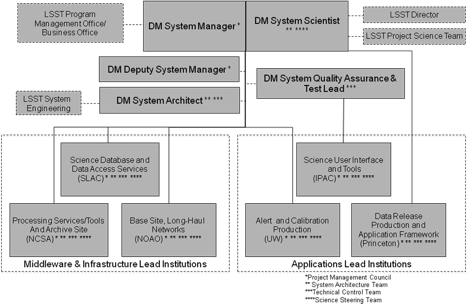
\includegraphics[width=0.8\textwidth]{images/fdphase}
\caption{ Data Management Final Design Phase Organization\label{fig:fdphase}}
\end{center}
\end{figure}





\subsection{References\label{sect:references}}
\vspace*{-1cm}
\renewcommand{\refname}{}
\bibliographystyle{gaia_aa}
\bibliography{gaia_livelink_valid,gaia_drafts,gaia_refs,gaia_books,gaia_refs_ads}

\subsection{Acronyms}
The following table has been generated from the on-line Gaia acronym list:
\newline\newline%decrement table counter so table sin doc start at 1.
\addtocounter{table}{-1}
\begin{longtable}{|l|p{0.8\textwidth}|}\hline 
\textbf{Acronym} & \textbf{Description}  \\\hline
API&Application Programming Interface \\\hline
CU&Coordination Unit (in DPAC) \\\hline
DM&Data Management (LSST) \\\hline
DPAC&Data Processing and Analysis Consortium \\\hline
DPACE&Data Processing and Analysis Consortium Executive \\\hline
ECSS&European Cooperation for Space Standardisation \\\hline
ESA&European Space Agency \\\hline
ESAC&European Space Astronomy Centre (VilSpa) \\\hline
ESF&European Science Foundation \\\hline
ESTEC&European Space research and TEchnology Centre (ESA) \\\hline
FOP&Flight Operation Procedure (Plan) \\\hline
GIS&(Astrometric) Global Iterative Solution \\\hline
IOA&Institute of Astronomy (Cambridge; also denoted IOA) \\\hline
LDAP&Lightweight Directory Access Protocol \\\hline
LSST&Large Synoptic Surrvey Telescope \\\hline
LTD&LSST the Docs \\\hline
LaTeX&(Leslie) Lamport TeX (document markup language and document preparation system) \\\hline
MDB&Main Database \\\hline
MOC&Mission Operations Centre \\\hline
NASA&National Aeronautics and Space Administration (USA) \\\hline
PR&Progress Report \\\hline
QA&Quality Assurance \\\hline
SDSS&Sloan Digital Sky Survey \\\hline
SOC&Science Operations Centre \\\hline
SVN&SubVersioN \\\hline
TOC&Table of Contents \\\hline
USA&United States of America \\\hline
WP&Work Package \\\hline
XMM&X-ray Multi-mirror Mission (ESA; officially known as XMM-Newton) \\\hline
\end{longtable} 
 % generated by the acronyms.csh (GaiaTools)


\end{document}
